We now investigate the CFL condition of the Lax-Friedrichs program from our previous report. Here, we show the results of the Lax-Friedrich for various values of $\Delta t/\Delta x$, given epsilon=0.1, alpha=$\Delta x/\Delta t$, xSteps=100, Tend=10. 

\FloatBarrier
\begin{figure}
\begin{center}
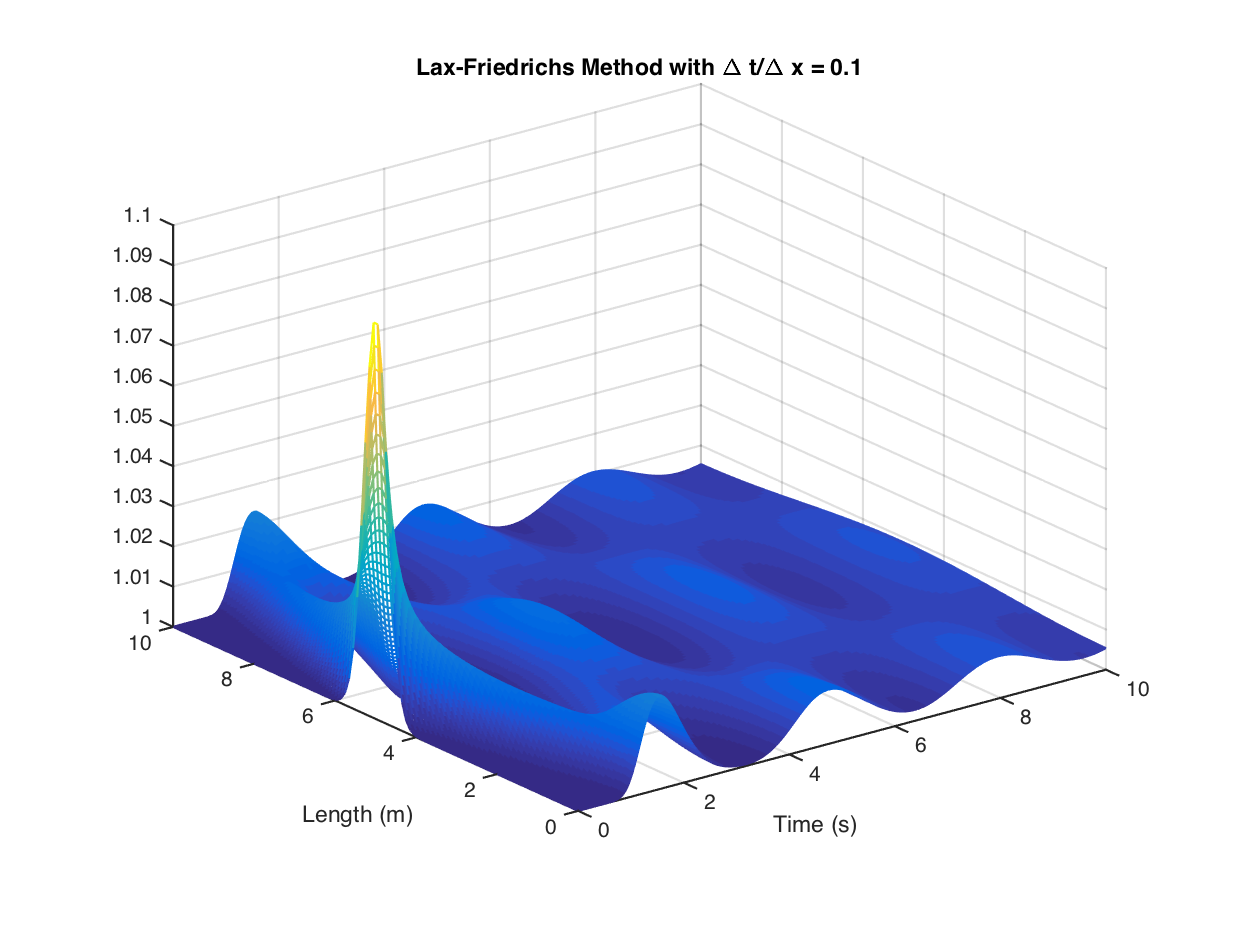
\includegraphics[scale=0.6]{lax01.eps}
\caption{Stable for $\Delta t/\Delta x=0.1$}
\label{reg}
\end{center}
\end{figure}

\begin{figure}
\begin{center}
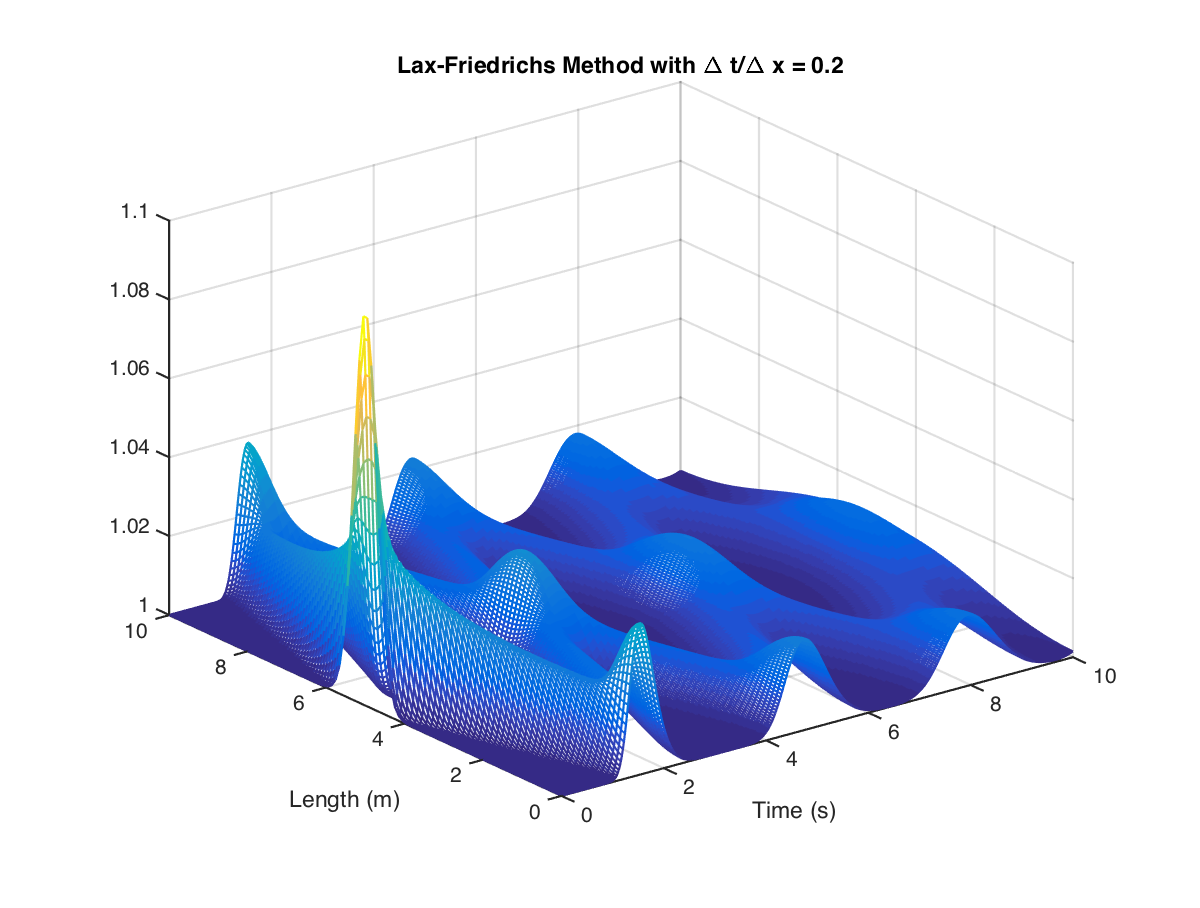
\includegraphics[scale=0.6]{lax02.eps}
\caption{Stable for $\Delta t/\Delta x=0.2$}
\label{reg}
\end{center}
\end{figure}

\begin{figure}
\begin{center}
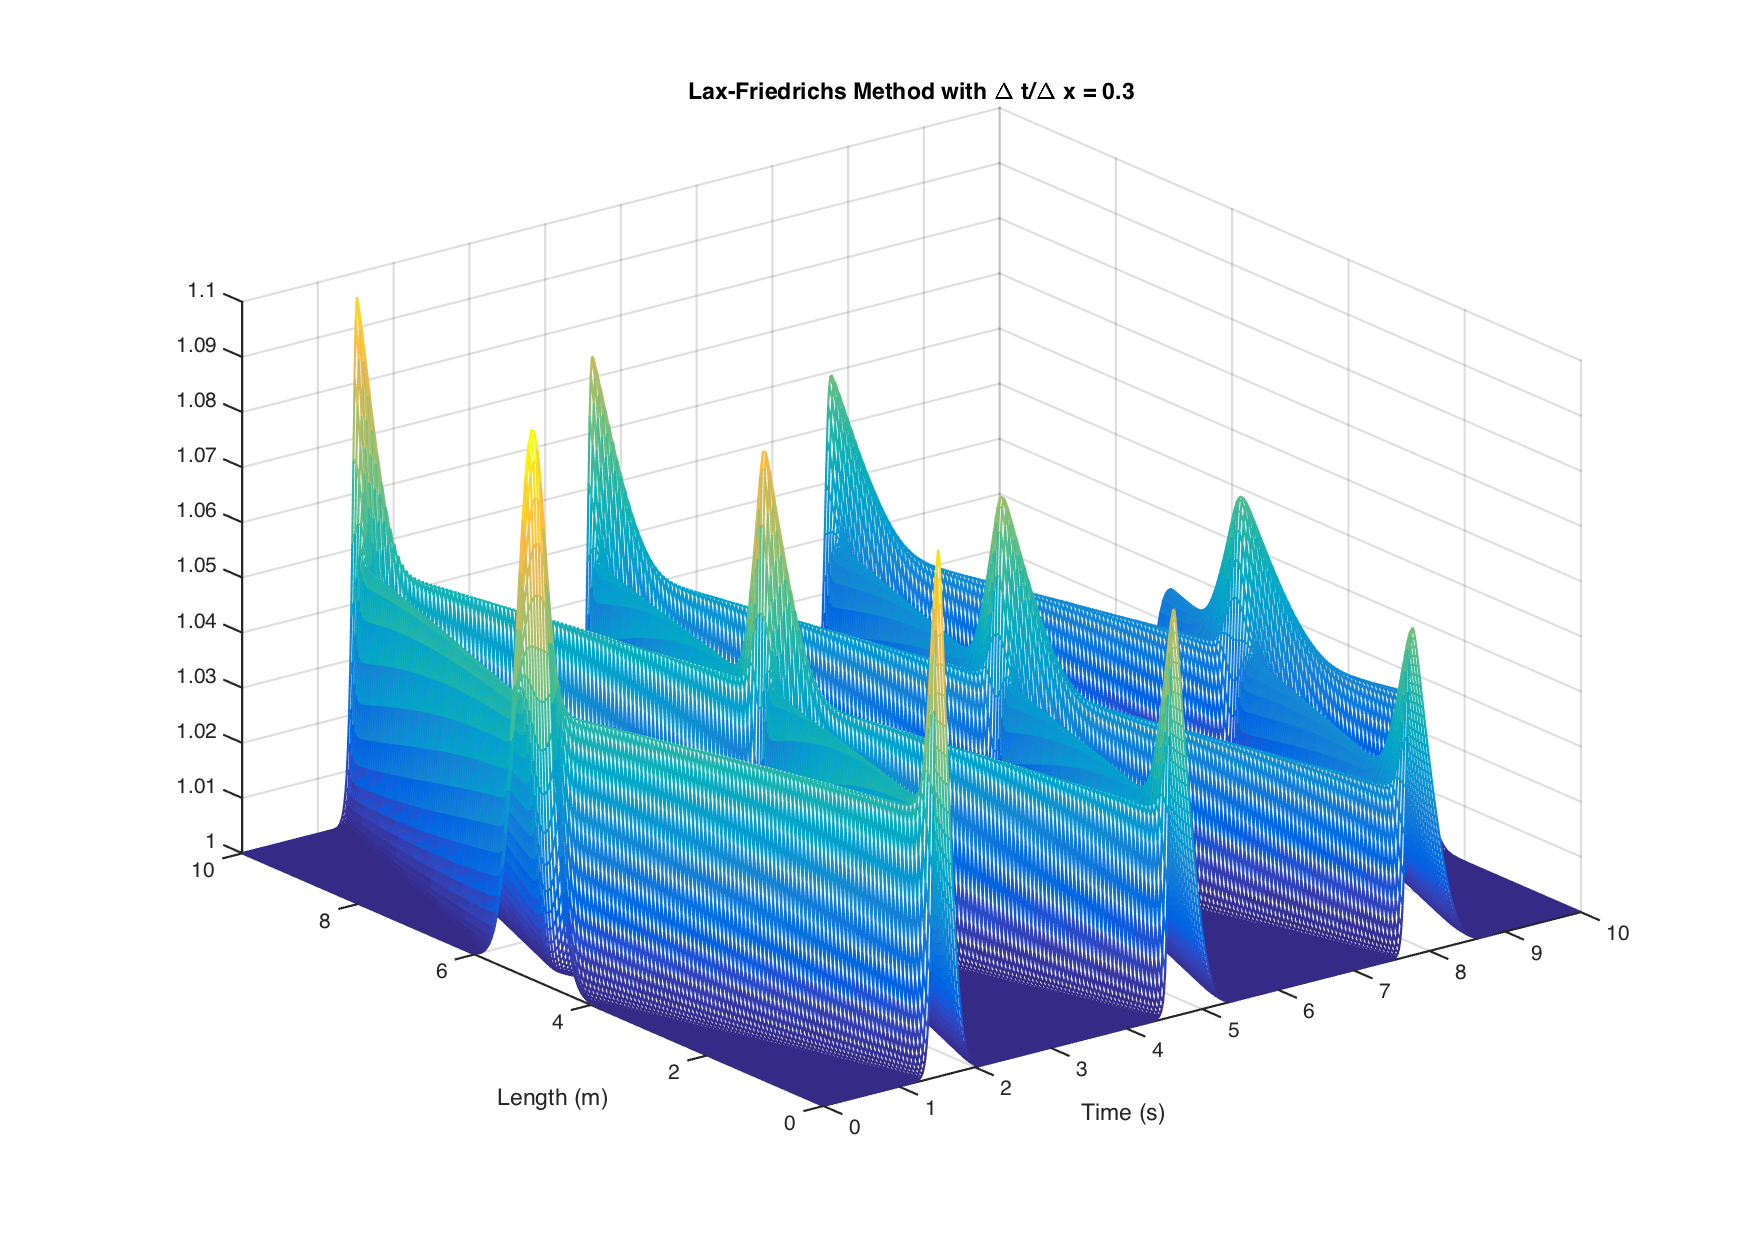
\includegraphics[scale=0.6]{lax03.eps}
\caption{Stable for $\Delta t/ \Delta x=0.306$ and $\Delta x = 200$}
\label{reg}
\end{center}
\end{figure}

\begin{figure}
\begin{center}
\includegraphics[scale=0.6]{lax307.eps}
\caption{Unstable for $\Delta t /\Delta x=0.307$}
\label{reg}
\end{center}
\end{figure}

As we can see, in our problem, the Lax-Friedrichs method becomes unstable at $\Delta t/\Delta x=0.307$. Another thing that is seen is that that the smaller $\Delta t/\Delta x$ is (the larger $\Delta x$ is compared to $\Delta t$), the larger the wave dampening. 

\FloatBarrier
\begin{figure}
\begin{center}
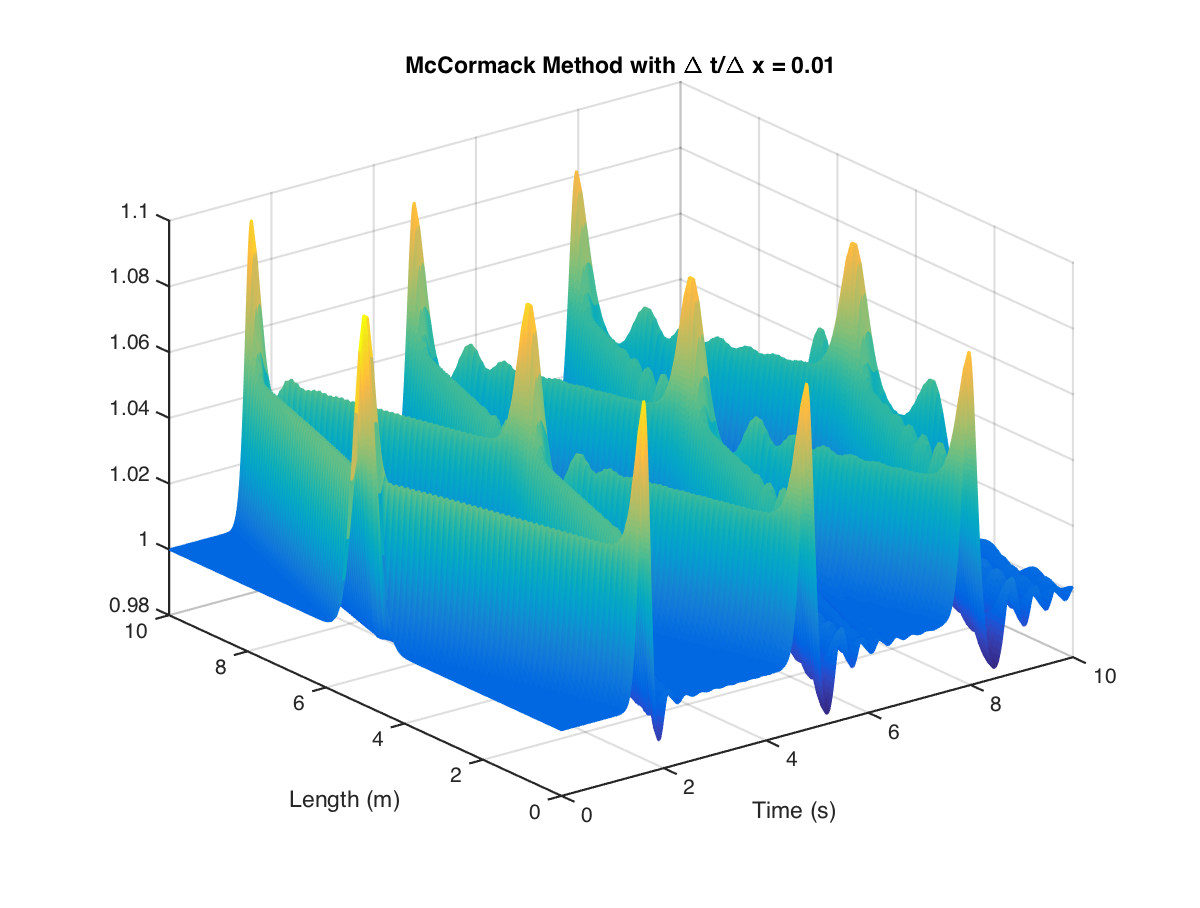
\includegraphics[scale=0.6]{mccormack001.eps}
%\caption{Stable for $\Delta t/\Delta x=0.1$}
\label{reg}
\end{center}
\end{figure}

\begin{figure}
\begin{center}
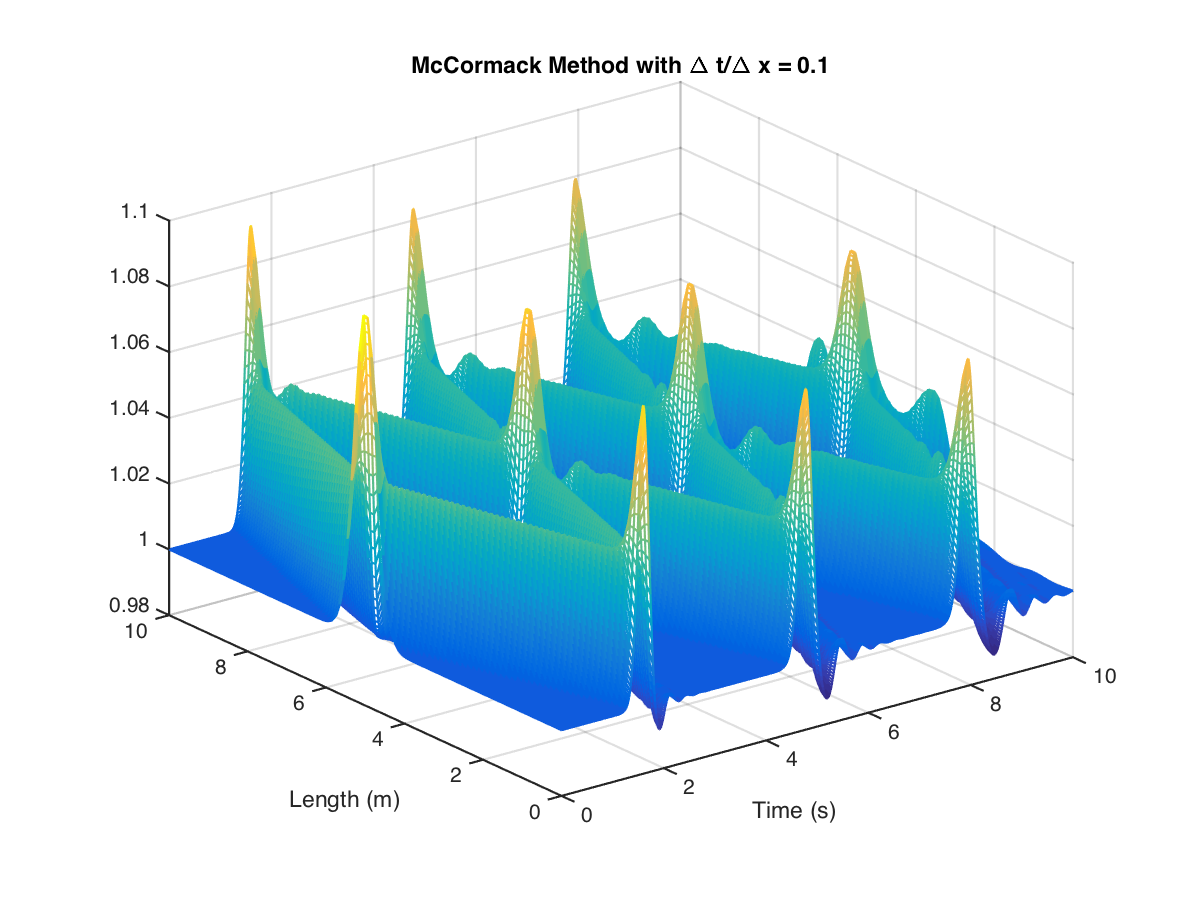
\includegraphics[scale=0.6]{mccormack01.eps}
%\caption{Stable for $\Delta t/\Delta x=0.2$}
\label{reg}
\end{center}
\end{figure}

\begin{figure}
\begin{center}
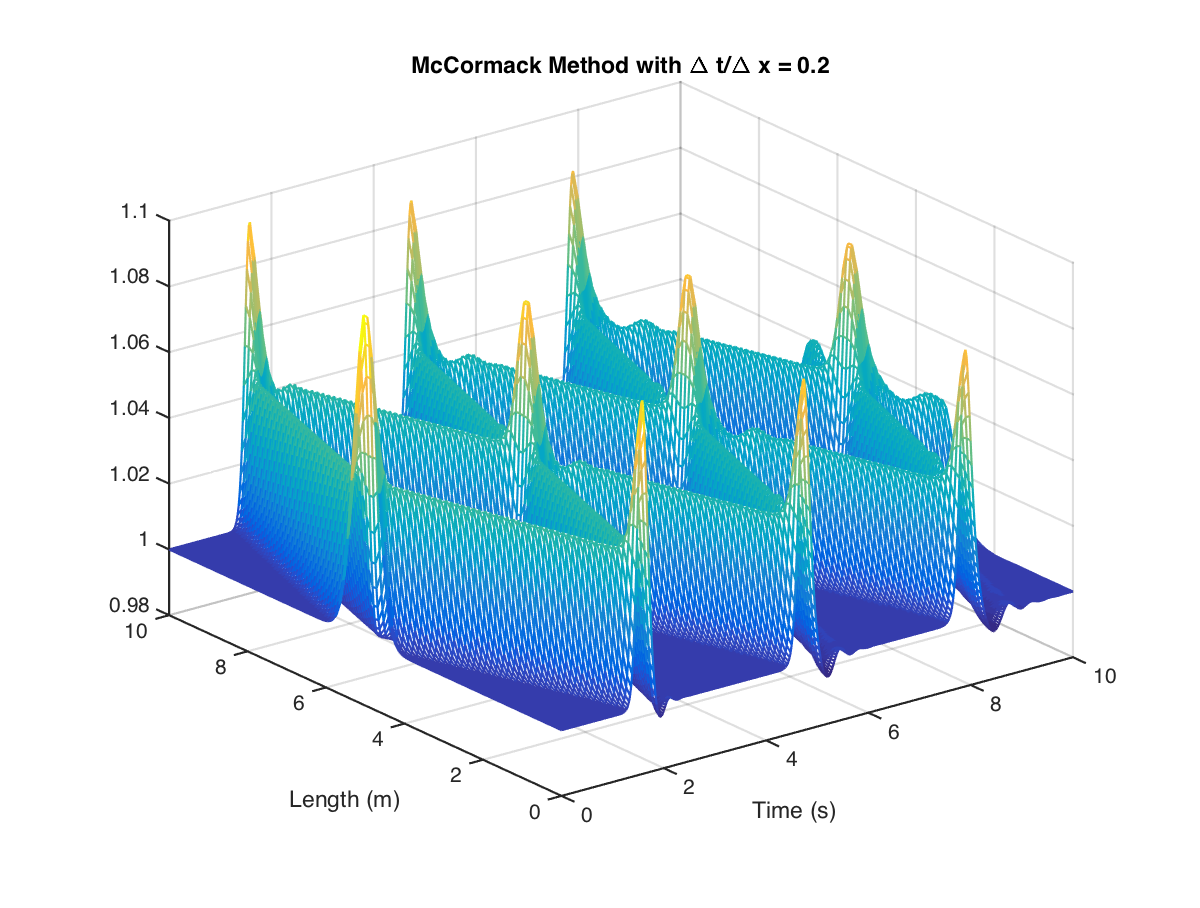
\includegraphics[scale=0.6]{mccormack02.eps}
%\caption{Stable for $\Delta t/ \Delta x=0.306$}
\label{reg}
\end{center}
\end{figure}

\begin{figure}
\begin{center}
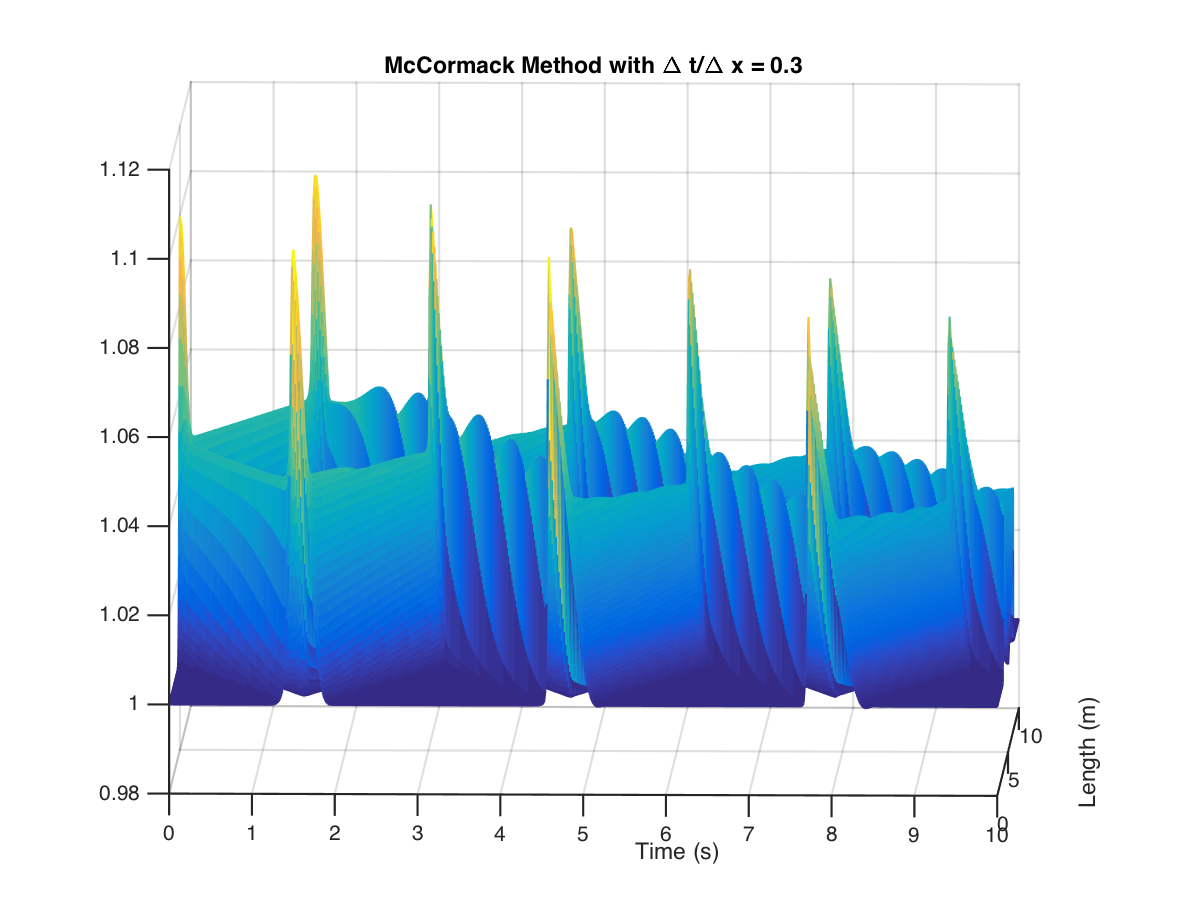
\includegraphics[scale=0.6]{mccormack03side.eps}
%\caption{Unstable for $\Delta t /\Delta x=0.307$}
\label{reg}
\end{center}
\end{figure}
